\documentclass[12pt]{article}
\usepackage{geometry}
\usepackage{graphicx} % 插图
\usepackage{float} % 插图位置固定
\usepackage{amsmath} % 文字加粗
\usepackage[UTF8]{ctex} %中文宏包
\setCJKmainfont{SimSun}
\usepackage{fontspec} %引入字体设置宏包
\setmainfont{Times New Roman}
\usepackage{indentfirst} %首行缩进
\usepackage{listings} %代码
\usepackage{color} %字体颜色
\usepackage{subfigure}  %插入多图时用子图显示的宏包

\usepackage{minted} %代码
\usemintedstyle{vs}


%\usepackage{fancyhdr} %页眉页脚
%\pagestyle{fancy} 
%\fancyhf{}
%\lhead{数字图像处理}
%\chead{Noise Reduction Using a Median Filter}
%\rhead{张青铭 \quad 3200105426}
%\renewcommand{\headrulewidth}{0pt}
%图片路径
\graphicspath{ {figures/} }

%页面格式
\geometry{a4paper,
left=20mm,
right=20mm,
top=20mm,
bottom=20mm }

\title{{\Huge{\textbf{数字图像处理}}}\\Pro10-2\quad  Global Thresholding}
\author{信息与电子工程学院\quad 信息工程 \quad 3200105426\\张青铭}
\date{\today}

\begin{document}
\maketitle
\section{实验任务}
(1)设计一个全局阈值处理程序,复现课本第十章第三节中的全局阈值处理操作,将灰度图输出为一个二值图像;

(2)下载合适图片进行实验;
\section{算法设计}
我们要设计的是自动估计阈值的算法,使用迭代以达到目的。算法如下:

1.为全局阈值T选择一个初始估计值;

2.通过下式用T分割图像,产生两组像素:G1由灰度值大于T的所有像素组成,G2由所有灰度值小于等于T的像素组成;
$$g(x,y)=\begin{cases}1&f(x,y)>T\\ 0&f(x,y)\leq T\end{cases}$$

3.对G1和G2的像素分别计算灰度均值m1和m2;

4.计算得到一个新的阈值T

5.迭代2-4,直到T小于$\Delta$T。
\section{代码实现}
\begin{minted}[frame=lines,tabsize=4,python3,baselinestretch=0.85]{matlab}
%% mian
clc;clear;close all;
I =imread('Fig1043.tif');
level =global_threshold(I);           
J = imbinarize(I,level);    
subplot(121)
imshow(I);
title('original image');
subplot(122)
imshow(J);
title('after global threshold');
%% function
function level =global_threshold(I)
I = im2double(I); 
[M,N] = size(I);
T0 = 0.001;         
T1 = (max(max(I)) +min(min(I)))/2;   
columns1 = 1;
columns2 = 1;
while 1
	for i = 1:M
		for j = 1:N
			if I(i,j)>T1
				G1(columns1) = I(i,j);  
				columns1 = columns1 + 1;
			else	
				G2(columns2) = I(i,j); 
				columns2 = columns2 + 1;
			end
		end
	end
	ave1 = mean(G1);
	ave2 = mean(G2);
	T2 = (ave1 + ave2)/2;  
	if abs(T2 - T1)<T0        
		break;
	end
	T1 = T2;
	columns1 = 1;
	columns2 = 1;
end
level = T2;
end
\end{minted}

\section{实验结果}
分别选择了两组灰度图像进行实现,效果如下:
\begin{figure}[H]
	\centering
	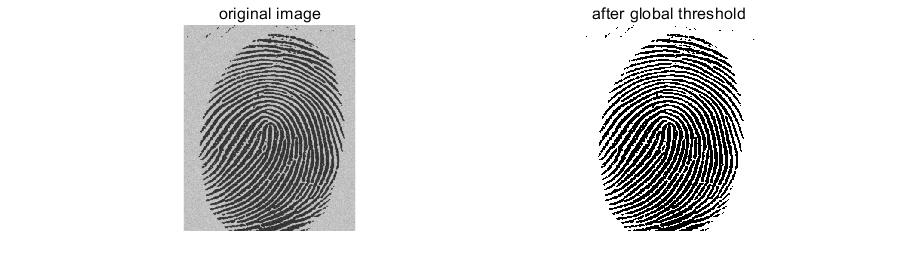
\includegraphics[width=1\linewidth]{figures/1}
	\caption{第一组}
\end{figure}
\begin{figure}[H]
	\centering
	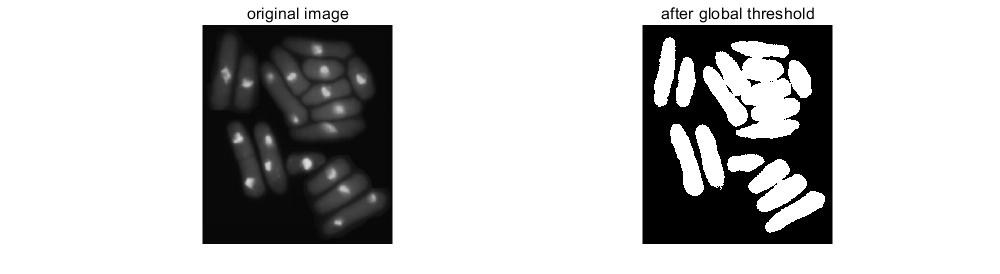
\includegraphics[width=1\linewidth]{figures/2}
	\caption{第二组}
\end{figure}

对于以上两张灰度图,可见经过全局阈值处理后,图片自动化处理为了二值化黑白图像。
\section{总结}
本次实验我对灰度图像的阈值处理操作进行了实验练习,实现了对不同灰度图像的阈值自动化计算,并且输出为二值图。
\end{document}
